\documentclass[default]{beamer}
\setbeamertemplate{navigation symbols}{}

\usetheme{Frankfurt}
%\useoutertheme{infolines}
\usecolortheme{beaver}

\usepackage[utf8]{inputenc}					% Выбор языка и кодировки
\usepackage[english, russian]{babel}	% Языки: русский, английский
\usepackage{csquotes}
\usepackage{tikz}
\usetikzlibrary{arrows,shapes,calc}
\usepackage{animate}
\usepackage{fp}
\usepackage{textpos}
				

\graphicspath{{../../images/}} 			% Пути к изображениям

\makeatletter
\setbeamertemplate{footline}
{
	\leavevmode%
	\hbox{%
		\begin{beamercolorbox}[wd=.333333\paperwidth,ht=2.25ex,dp=1ex,center]{author
				in head/foot}%
			\usebeamerfont{author in
				head/foot}\insertshortauthor~~\beamer@ifempty{\insertshortinstitute}{}{(\insertshortinstitute)}
		\end{beamercolorbox}%
		\begin{beamercolorbox}[wd=.333333\paperwidth,ht=2.25ex,dp=1ex,center]{title in
				head/foot}%
			\usebeamerfont{title in head/foot}\insertshorttitle
		\end{beamercolorbox}%
		\begin{beamercolorbox}[wd=.333333\paperwidth,ht=2.25ex,dp=1ex,right]{date in
				head/foot}%
			\usebeamerfont{date in head/foot}\insertshortdate{}\hspace*{2em}
			\insertframenumber{}\hspace*{2ex} 
		\end{beamercolorbox}
	}%
	\vskip0pt%
}


\begin{document}
	
	\title[Методы и технологии ИИ]{Методы и технологии искусственного интеллекта}
	\author[Осипов, Панов]{\textbf{Г.С. Осипов\\А.И. Панов}}
	\institute[ФИЦ ИУ РАН]{Федеральный исследовательский центр <<Информатика и управление>>\\Российской академии наук}
	\date{21 декабря 2016} 
	
	{
	\setbeamertemplate{headline}{}
	\begin{frame}
		
		\titlepage
		\centering
		\href{mailto:gos@isa.ru}{gos@isa.ru}
		
		
\includegraphics[width=100pt]{misc/logos/ras.png} \hspace{10pt}
		
\includegraphics[width=80pt]{misc/logos/frccsc.png} \hspace{10pt}
		
\includegraphics[width=40pt]{misc/logos/raai.png}
	\end{frame}
	}	

	\section{Направления ИИ}
	\subsection{1.4}
	\begin{frame}
		\frametitle{Современный ИИ}
		\Large
		\begin{itemize}
			\item \textbf{Середина 70-х гг.} --- качественный скачок в работах по искусственному интеллекту.
			\item Появление  первых прикладных систем, использующих знания для решения различных всё более сложных задач.
			\item \textbf{Середина 2000-х годов} --- резкое повышение интереса к практическим приложениям одного из направлений ИИ --- машинного обучения.
		\end{itemize}
	\end{frame}

	\subsection{3.1}
	\begin{frame}
		\frametitle{Основные направления ИИ}
		\centering
		\footnotesize
		\makebox[0.8\textwidth][c]{
			\begin{tikzpicture}
				\node[ellipse, minimum width = 100, minimum height = 50, fill=blue!20, align=center] (d1) {Искусственный\\интеллект};
				
				\node[rounded corners=5pt,draw,color=blue!20, very thick,text=black] (d2) at (-4,2) {
					\begin{minipage}[c][33pt]{100pt}
						\centering
						\textbf{Приобретение знаний, анализ данных и порождение гипотез}
					\end{minipage}
				};
				\node[rounded corners=5pt,draw,color=blue!20, very thick,text=black] (d3) at (-4,0.5) {
					\begin{minipage}[c][20pt]{80pt}
					\centering
					\textbf{Моделирование рассуждений}
					\end{minipage}
				};
	
				\node[rounded corners=5pt,draw,color=blue!20, very thick,text=black] (d4) at (-4,-0.7) {
					\begin{minipage}[c][20pt]{80pt}
					\centering
					\textbf{Многоагентные системы}
					\end{minipage}
				};
			
				\node[rounded corners=5pt,draw,color=blue!20, very thick,text=black] (d5) at (-4,-2.3) {
					\begin{minipage}[c][43pt]{110pt}
					\centering
					\textbf{Обработка естественного языка, пользовательский интерфейс и модели пользователя}
					\end{minipage}
				};
			
			
				\node[rounded corners=5pt,draw,color=blue!20, very thick,text=black] (d6) at (4,2) {
					\begin{minipage}[c][33pt]{120pt}
					\centering
					\textbf{Динамические интеллектуальные системы и планирование поведения}
					\end{minipage}
				};
				\node[rounded corners=5pt,draw,color=blue!20, very thick,text=black] (d7) at (4,0.5) {
					\begin{minipage}[c][20pt]{80pt}
					\centering
					\textbf{Представление знаний}
					\end{minipage}
				};
				
				\node[rounded corners=5pt,draw,color=blue!20, very thick,text=black] (d8) at (4,-0.7) {
					\begin{minipage}[c][20pt]{100pt}
					\centering
					\textbf{Нечеткие модели и мягкие вычисления}
					\end{minipage}
				};
				
				\node[rounded corners=5pt,draw,color=blue!20, very thick,text=black] (d9) at (4,-2.3) {
					\begin{minipage}[t][20pt]{110pt}
					\centering
					\textbf{Инструментальные средства и технологии}
					\end{minipage}
				};
				
				\draw[->,rounded corners=10pt, very thick, blue!20](d1)[xshift=-10] |- (d2.east);
				\draw[->,rounded corners=10pt, very thick, blue!20](d1)[xshift=10] |- (d6.west);
				
				\draw[->,rounded corners=10pt, very thick, blue!20](d1)[xshift=-10] |- (d5.east);
				\draw[->,rounded corners=10pt, very thick, blue!20](d1)[xshift=10] |- (d9.west);
				
				\draw[->,rounded corners=10pt, very thick, blue!20](d1) |- (d3.east);
				\draw[->,rounded corners=10pt, very thick, blue!20](d1) |- (d7.west);
				
				\draw[->,rounded corners=10pt, very thick, blue!20](d1.south west) |- (d8.west);
				\draw[->,rounded corners=10pt, very thick, blue!20](d1.south east) |- (d4.east);
			\end{tikzpicture}
		}
	\end{frame}

	\subsection{3.2}
	\begin{frame}
		\frametitle{Приобретение знаний, анализ данных и автоматическое порождение гипотез}
		
		\textbf{Цель}: создание методологий, технологий и программных средств обнаружения и переноса компетентности   в базы знаний.
		\par\medskip
		\centering
		\tikz[baseline]{
			\small
			\node[fill=yellow, rounded corners=5pt, minimum width=300, minimum height = 150] (k1) {
				\begin{minipage}[t][150pt]{300pt}
					\centering
					\textbf{Методы приобретения знаний:}
				\end{minipage}
				
			};
			
			\node[rounded corners=5pt, minimum width=280, minimum height = 50, text width= 250, text centered,fill=white] (k2) at (0, 0.85) {
				\begin{minipage}[t][60pt]{250pt}
					\centering
					\textbf{Машинное обучение и обучение по примерам} (методы построения деревьев решений,  индуктивные методы построения правил;  статистические методы, в частности, Байесовские  сети; метод ближайших соседей, искусственные нейронные сети)
				\end{minipage}
				
			};
		
			\node[rounded corners=5pt, minimum width=280, minimum height = 10, text width= 250, text centered,fill=white] (k2) at (0,-0.9) {
				\begin{minipage}[t][10pt]{250pt}
					\centering
					\textbf{Приобретение знаний из текстов}
				\end{minipage}
				
			};
		
			\node[rounded corners=5pt, minimum width=280, minimum height = 20, text width= 250, text centered,fill=white] (k2) at (0, -2) {
				\begin{minipage}[t][20pt]{250pt}
					\centering
					\textbf{Прямые методы приобретения знаний (автоматизированный диалог с экспертами)}
				\end{minipage}
				
			};
		}
	\end{frame}

	\subsection{3.3}
	\begin{frame}
		\frametitle{Представление знаний}
		
		\textbf{Предмет}:  разработка языков и программных средств   для описания экспертных и эмпирических знаний. 
		\par\medskip
		\textbf{Содержание}:
		\begin{itemize}
			\item семантические сети, системы фреймов, системы правил (продукционные системы) и их гибриды;
			\item логики пространства и времени;
			\item онтологии – способ обмена знаниями;
			\item дескриптивные логики (теория баз знаний и онтологий).
		\end{itemize}
		\begin{columns}
			\begin{column}{0.45\textwidth}
				\includegraphics[width=\textwidth,page=3]{examples/causnet/caus_net}
			\end{column}
			\begin{column}{0.45\textwidth}
				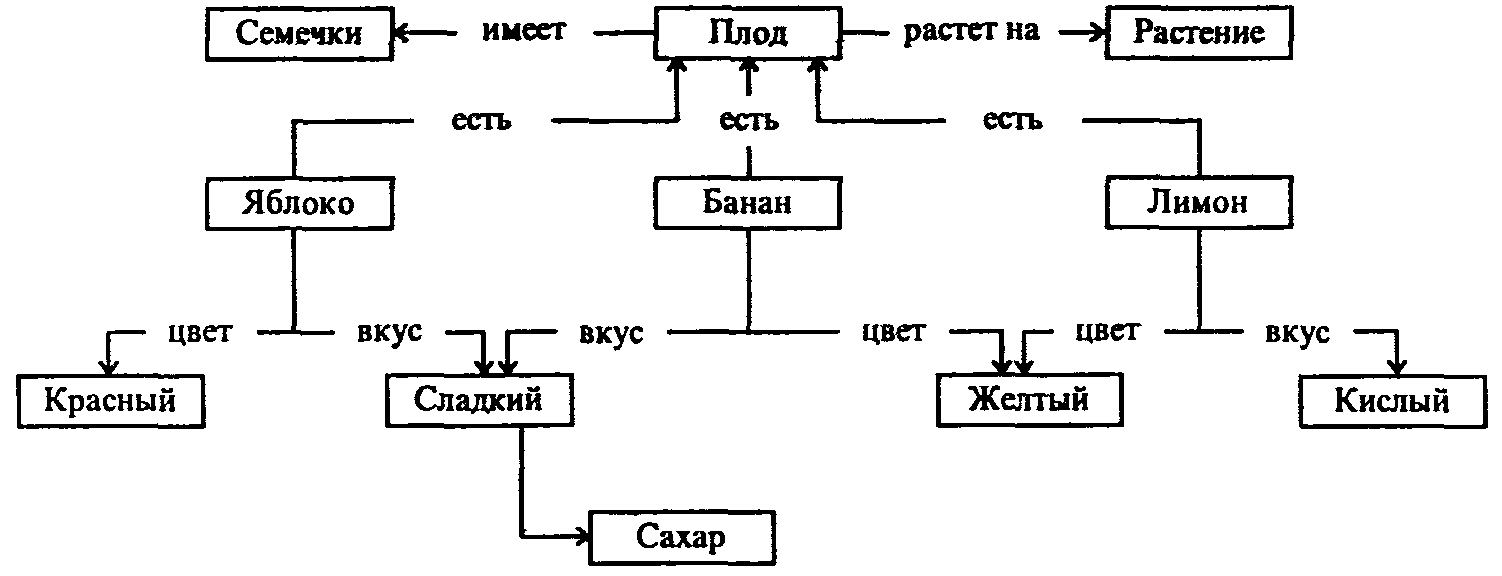
\includegraphics[width=\textwidth]{misc/presentations/semnet1.png}
			\end{column}
		\end{columns}	
	\end{frame}

	\subsection{3.4}
	\begin{frame}
		\frametitle{Автоматизация  рассуждений}
		
		Методы индукции, абдукции и аналогии, аргументации, рассуждения на основе прецедентов, на основе ограничений, рассуждения о действиях и изменениях, рассуждения с неопределенностью, немонотонные рассуждения.
		\par\medskip
		\tikz[baseline]{
			\node[fill=blue!20, rounded corners=5pt, anchor=base] (t1) {\textbf{Немонотонные рассуждения}};
		}
		связаны с поиском эмпирических зависимостей в данных, обучением по примерам и рассуждениями в эмпирических  теориях. Выделились в самостоятельный раздел логики.
		\par\medskip
		\tikz[baseline]{
			\node[fill=blue!20, rounded corners=5pt, anchor=base] (t2) {\textbf{Рассуждения о действиях}};
		}
		исследуют связь  действий и эффектов действий (результатов действий).
		\par\medskip
		\tikz[baseline]{
			\node[fill=blue!20, rounded corners=5pt, anchor=base] (t3) {\textbf{Рассуждения с неопределенностью}};
		}
		--- использование  Байесовского  формализма в моделях рассуждений. 
		
	\end{frame}

	\subsection{3.5}
	\begin{frame}
		\frametitle{Многоагентные системы}
		
		Изучаются интеллектуальные программные агенты, их коалиции и поведение.
		
		\par\medskip
		\textbf{Интеллектуальный программный  агент} --- программная система, обладающая автономностью, социальными чертами, реактивностью и активностью.
		
		\par\medskip
		\textbf{Основные проблемы}: коммуникация интеллектуальных агентов, разработка языков для этой цели, координация поведения  агентов, распределение ролей в коалициях агентов, коллективное поведение агентов.
		\par\medskip
		\textbf{Экспериментальным результатом исследования обучения агентов явилось то, что группа агентов лучше обучается решению сложных задач, чем индивидуально на тех же самых примерах.}
	\end{frame}

	\subsection{3.7}
	\begin{frame}
		\frametitle{Роботы и автономные системы}
		\Large
		\begin{itemize}
			\item Диалоговое взаимодействие коалиций мобильных роботов.
			\item Интерпретация команд, поступающих от человека.
			\item Качественные логики пространства-времени.
			\item Рассуждения, основанные на оценках.
		\end{itemize}
		\begin{columns}
			\begin{column}{0.45\textwidth}
				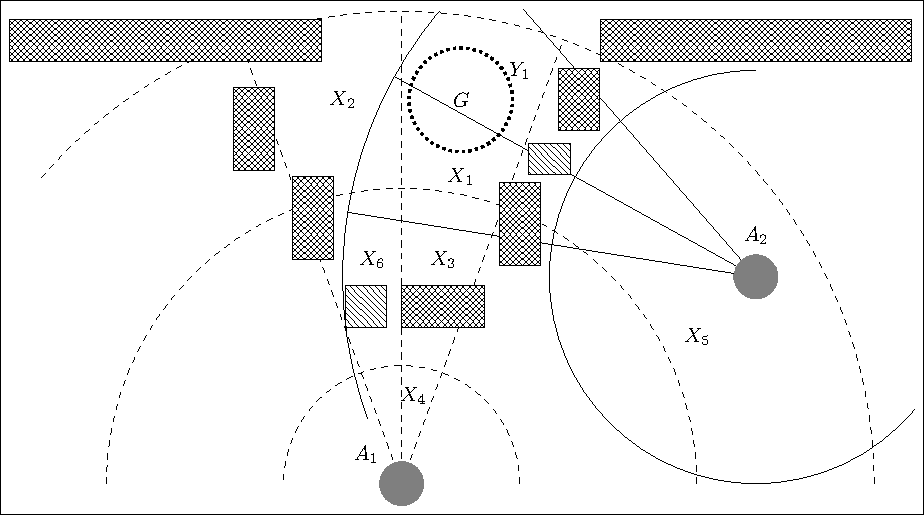
\includegraphics[width=\textwidth]{examples/representations/rita_ex_proc}
			\end{column}
			\begin{column}{0.45\textwidth}
				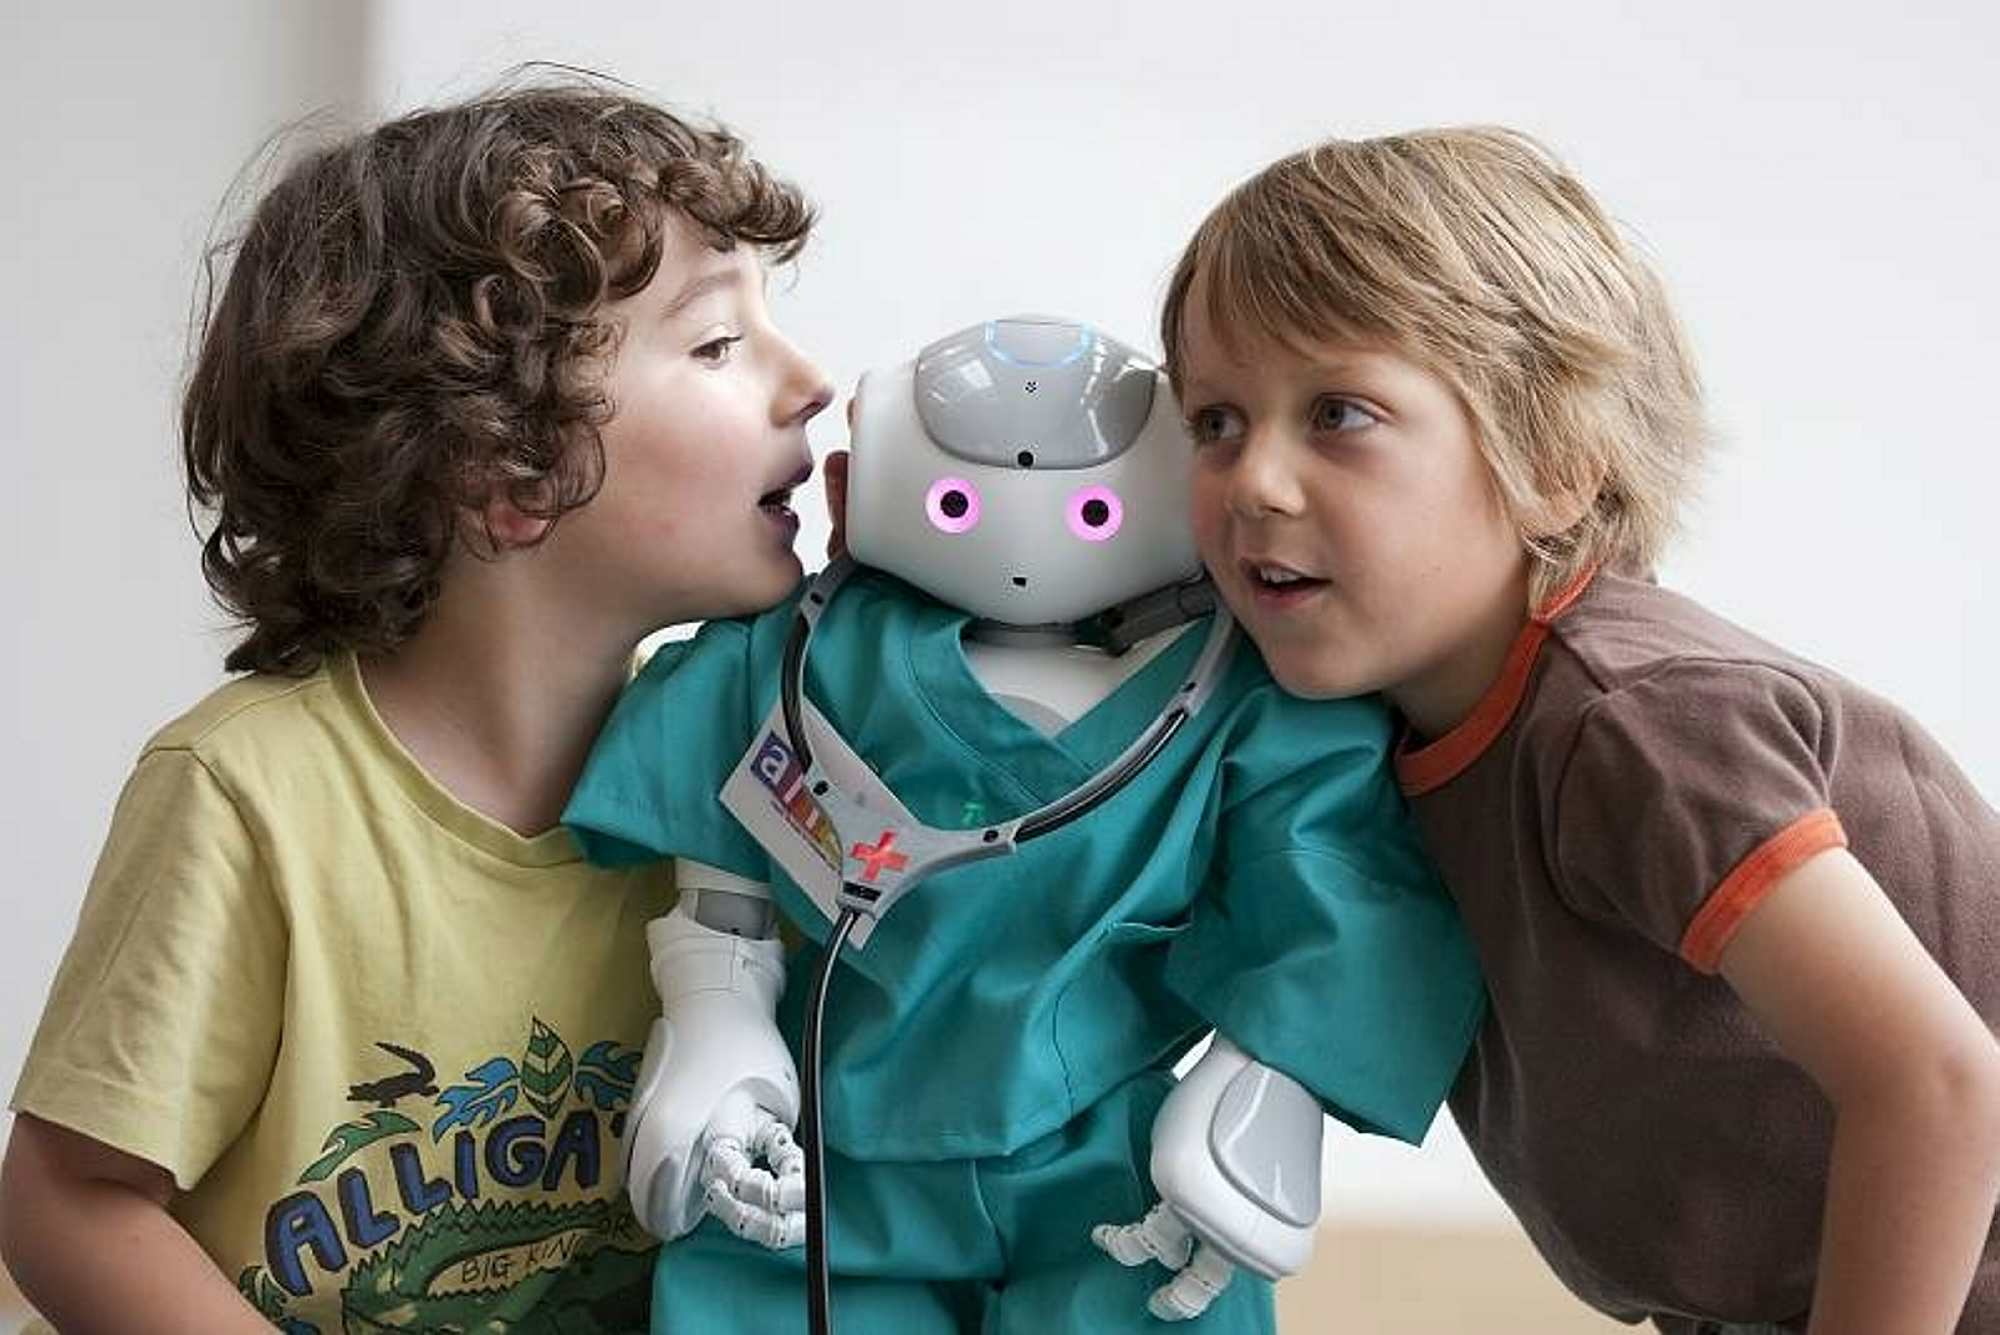
\includegraphics[width=\textwidth]{misc/presentations/nao_hri.jpg}
			\end{column}
		\end{columns}		
	\end{frame}

	\subsection{3.8}
	\begin{frame}
		\frametitle{Интеллектуальные динамические системы и автоматическое планирование поведения}
		
		\textbf{Результат интеграции} методов искусственного интеллекта с теорией динамических систем:
		\begin{itemize}
			\item планирование,
			\item моделирование,
			\item управление.
		\end{itemize}
		\textbf{Объект} --- сложные системы с неколичественными (логическими или лингвистическими) переменными состояния и динамикой, описываемой экспертными или эмпирическими правилами.
	\end{frame}

	%\subsection{3.9}
	\begin{frame}
		\frametitle{Обработка естественного языка, интерфейс и модели пользователя}
		\begin{itemize}
			\small
			\item Семантический поиск в больших массивах текстов:
			\begin{itemize}
				\footnotesize
				\item поиск документов (в полнотекстовой БД, в локальных и глобальных телекоммуникационных сетях);
				\item извлечение данных из текстов;
				извлечение знаний из текстов.
			\end{itemize}
			
			\item Обработка текстов: сегментация, классификация, кластеризация, аннотирование или реферирование текстов. Перевод. 
			\item Диалоговые системы: 
			\begin{itemize}
				\footnotesize
				\item интеллектуальные вопросно-ответные системы; 
				\item системы общения конечных пользователей с БД, предоставляющие  различные услуги (выполнение банковских операций по телефону, заказ товаров по каталогам); 
				\item голосовое управление техникой, кооперативное решение проблем (человек плюс интеллектуальная система).
			\end{itemize}
			
			\item Автоматическое обучение анализу текстов.
			
		\end{itemize}
		
	\end{frame}

	\subsection{3.10}
	\begin{frame}
		\frametitle{Нечеткие модели и мягкие вычисления}
		
		\Large 
		\begin{itemize}
			\item Нечеткие схемы вывода по аналогии;
			\item теория нечетких мер; 
			\item модели геометрических объектов;
			\item алгоритмы эволюционного моделирования с динамическими параметрами (например, время жизни и размер популяции);
			\item методы решения оптимизационных задач с использованием технологий генетического поиска, гомеостатических и синергетических принципов и элементов самоорганизации. 
		\end{itemize}
		
	\end{frame}

	\section{Перспективы ИИ}
	\subsection{4.1}
	\begin{frame}
		\frametitle{Перспективные направления ИИ}
		
		\begin{itemize}
			\item \textbf{Рассуждения, основанные на прецедентах}.
			\item \textbf{Рассуждения о пространстве} --- возрастающее значение для автономных мобильных устройств, анализа изображений (в частности, аэрофотоснимков), синтеза текстовых описаний по изображениям.
			\item \textbf{Методы машинного обучения и автоматического формирования гипотез} --- решение практических задач: от обнаружения  закономерностей в данных до повышения степени адаптивности различных технических устройств.
			\item Подходы, основанные на \textbf{технологии интеллектуальных агентов} перспективны при разработке больших программных систем.
			
		\end{itemize}
		
	\end{frame}

	\subsection{4.2}
	\begin{frame}
		\frametitle{Перспективные направления ИИ}
		
		\begin{itemize}
			\item \textbf{Влияние идей и методов ИИ на машинный анализ текстов на естественном языке} --- коснется  семантического анализа и методов синтаксического анализа --- в этой области оно проявится в учете модели мира и использовании знаний о предметной области  для уменьшения переборов  на более ранних стадиях анализа.
			\item \textbf{Понимание текста}.
			\item \textbf{Автоматическое планирование и управление поведением}. Область применения  - от бытовой  техники до беспилотных аппаратов для исследования глубокого космоса.
		\end{itemize}
		
	\end{frame}

	\subsection{4.3}
	\begin{frame}
		\frametitle{Когнитивное компьютерное моделирование}
		\small
		\begin{itemize}
			\item Новое направление в искусственном интеллекте.
			\item Основано на изучении нейрофизиологических процессов для описания формирования психических функций.
			\item В качестве модели используется знаковая картина мира и модель возврата возбуждения в первичные отделы коры головного мозга.
			\item Новые постановки задач:
			\begin{itemize}
				\item выдвижение новой цели,
				\item модели интроспекции и рефлексивного поведения,
				\item динамическое распределение ролей в коалиции.
			\end{itemize}
		\end{itemize}
		\centering
		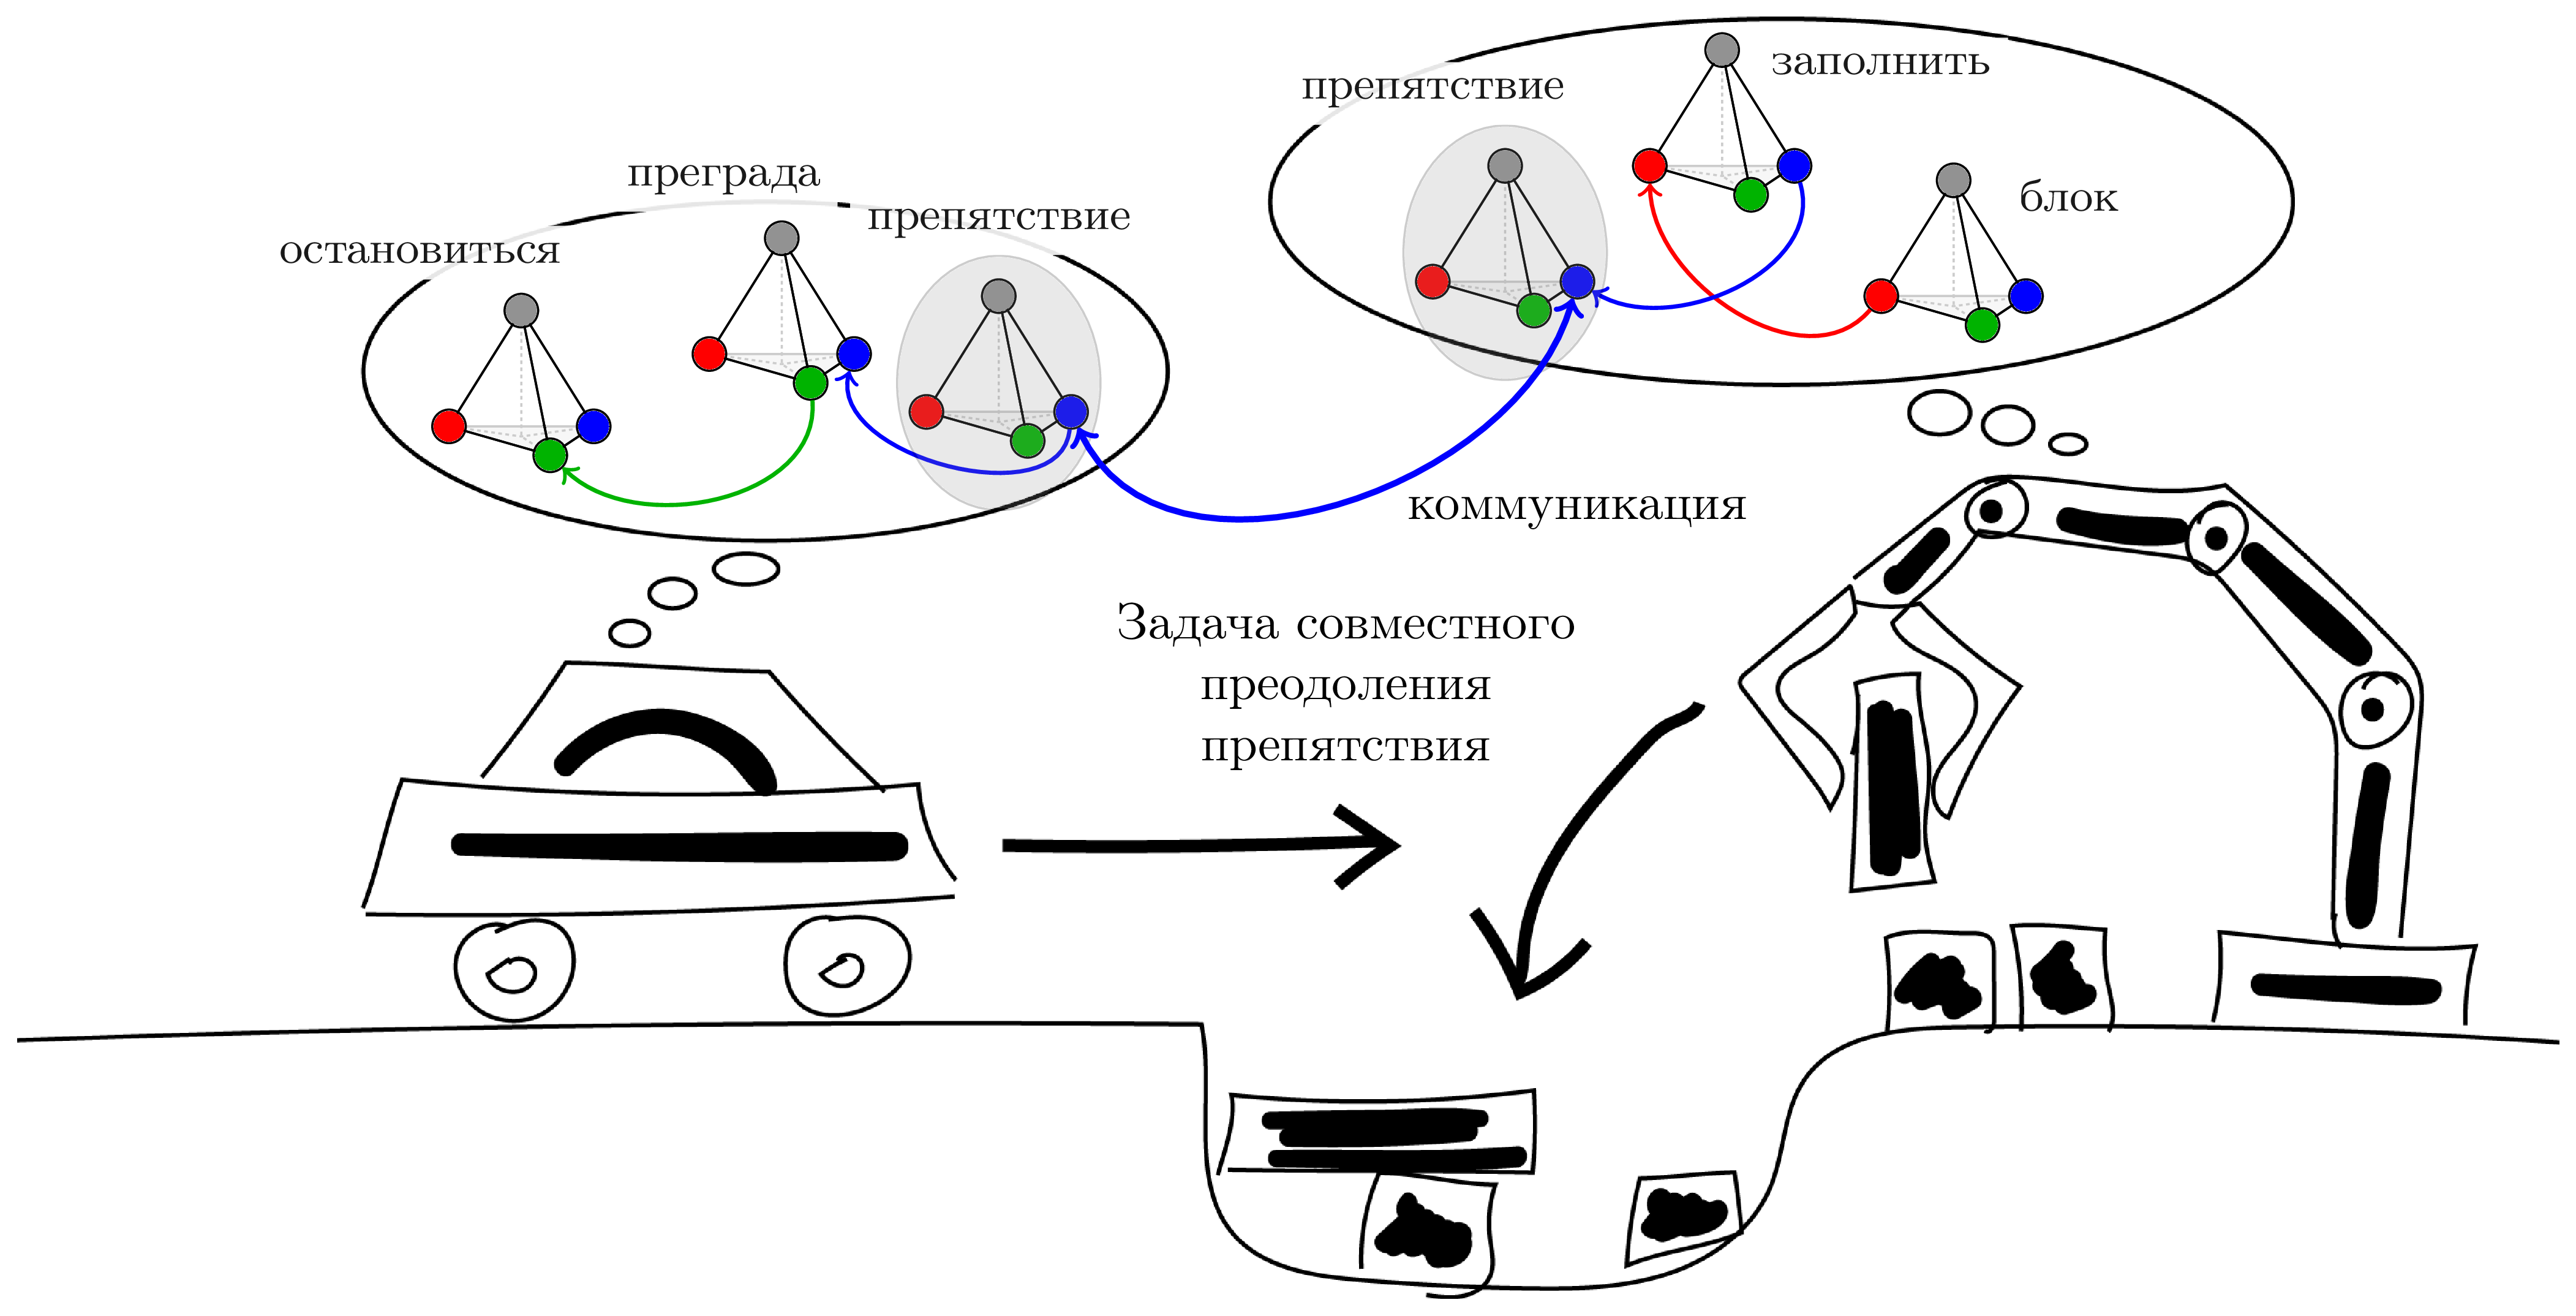
\includegraphics[width=0.45\textwidth]{examples/signs/robotic_signs.png}
	\end{frame}

	\section{Технологии ИИ}

	\subsection{5.6}
	\begin{frame}
		\frametitle{Системы и технологии ИИ в ФИЦ ИУ РАН}
		\Large
		\begin{itemize}
			\item Семантическая поисковая машина нового поколения EXACTUS. Машина работает с запросами на естественном языке.
			\item Неоднократно занимала первые места по релевантности поиска на соревнованиях поисковых 	машин \href{www.exactus.ru}{www.exactus.ru}.
		\end{itemize}
	\end{frame}

	\subsection{5.7}
	\begin{frame}
		\frametitle{Системы и технологии ИИ в ФИЦ ИУ РАН}
		\footnotesize
		\begin{itemize}
			\item Создана и реализована технология реляционно-ситуационного анализа неструктурированной, в том числе текстовой информации.
			\item На основе этой технологии и методов машинного обучения реализовано семейство поисково-аналитических систем, среди которых:
			\begin{itemize}
				\scriptsize 
				\item система прогнозирования социального стресса на основе анализа социальных медиа, 
				\item система интеллектуального поиска и анализа текстовой информации \textbf{Exactus Expert} --- предоставляет уникальные возможности для работы с научными текстами: семантический поиск и навигация , тематический анализ публикационной активности, оценка соответствия научных статей формальным требованиям, анализ научных направлений и коллективов, 
				\item \textbf{Exactus Patent} --- система интеллектуального поиска и анализа патентной информации, 
				\item \textbf{Exactus Like} --- система интеллектуального поиска заимствований в научных текстах, 
				\item \textbf{TextAppliance} --- программно-аппаратный комплекс интеллектуального поиска и анализа больших массивов текстов.
			\end{itemize}
		\end{itemize}
	\end{frame}

	\subsection{4.3}
	\begin{frame}
		\frametitle{Работы в  области автоматического планирования поведения и управления}
		
		\begin{itemize}
			\item Построена теория интеллектуальных динамических систем.
			\item Разработаны и реализованы алгоритмы планирования траектории беспилотных аппаратов.
			\item Разработаны методы группового взаимодействия в коалициях робототехнических систем
		\end{itemize}
		\begin{columns}
			\begin{column}{0.45\textwidth}
				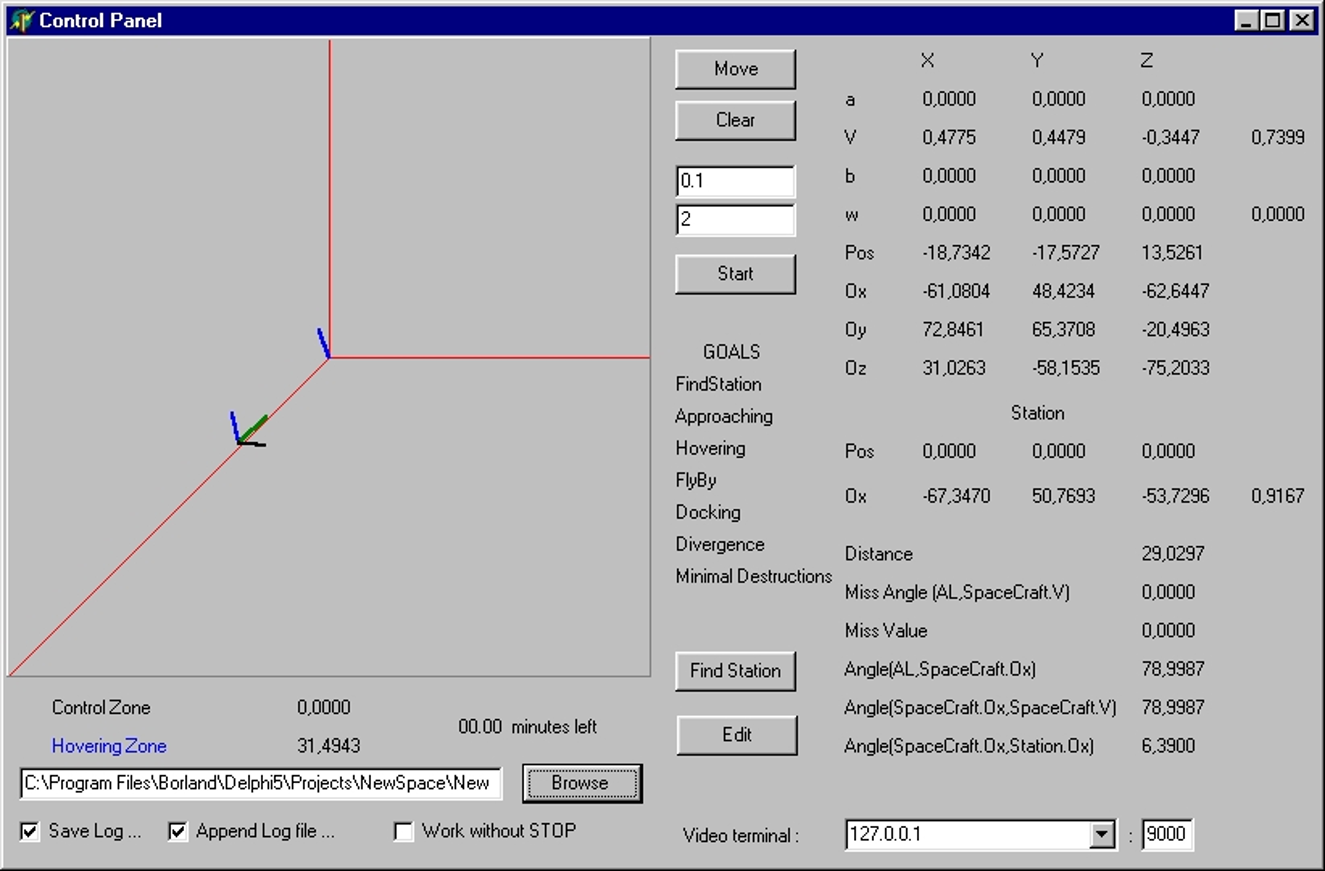
\includegraphics[width=\textwidth]{misc/control/space_control1.png}
			\end{column}
			\begin{column}{0.45\textwidth}
				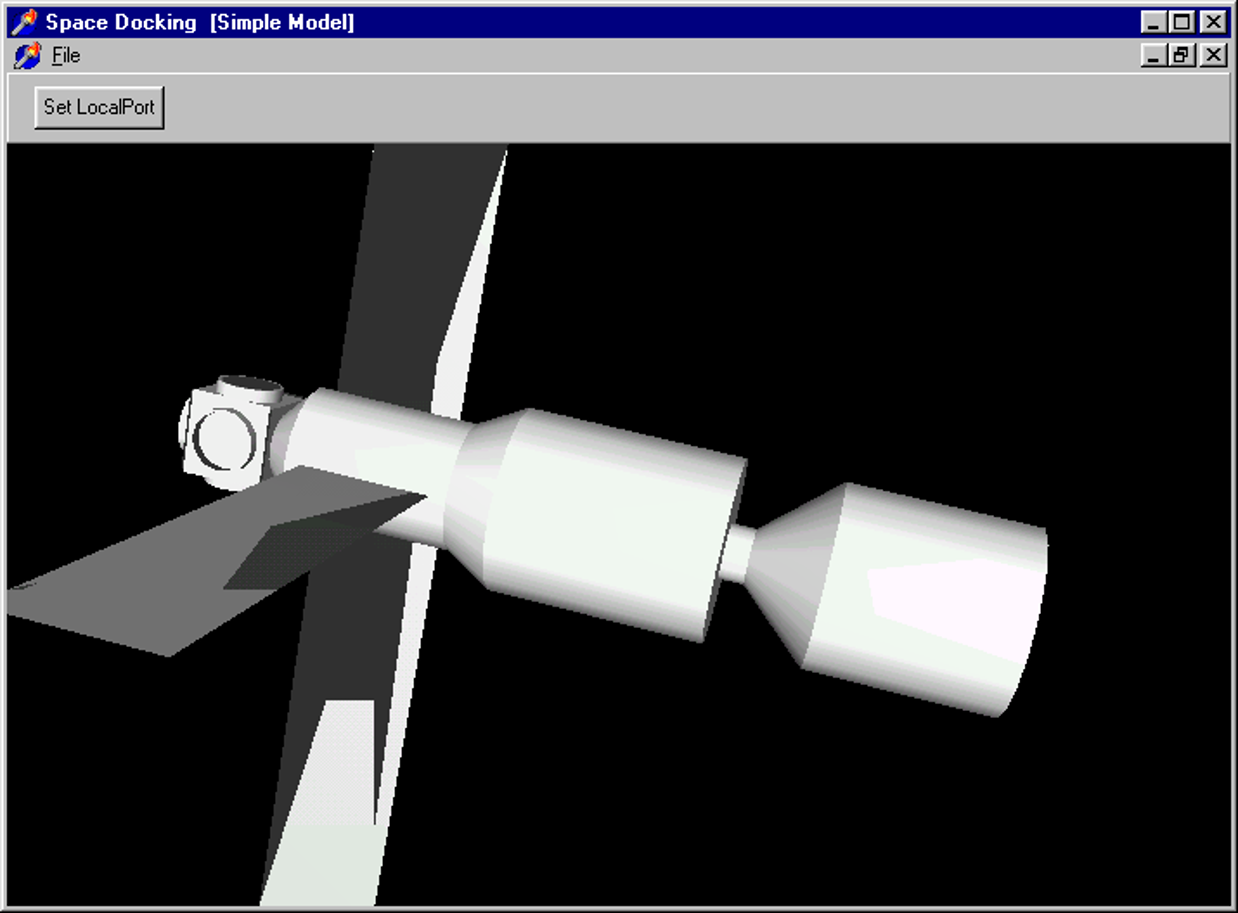
\includegraphics[width=\textwidth]{misc/control/space_control2.png}
			\end{column}
		\end{columns}
	\end{frame}

	\subsection{4.3}
	\begin{frame}
		\frametitle{Перспективные технологии ИИ}
		
		\begin{itemize}
			\item Экспертные системы диагностики, мониторинга и управления.
			\item Интегрированные среды поддержки методологии проектирования (SIMER+MIR).
			\item Моделирование бизнес --- процессов на основе систем бизнес-правил.
			\item Банковские системы, например,  анализ транзакций с целью выявления сомнительных операций и  мошенничества или обнаружение так называемого layering (лээринга) --- действия покупателя пакета акций, направленные на снижение цены этих акций посредством создания фиктивного предложения больших пакетов этих акций.
			\item Технологии интеллектуальных динамических систем.
			\item Технологии интеллектуального управления (подвижным составом железных дорог).
		\end{itemize}
		
	\end{frame}
	
	\subsection{4.3}
	\begin{frame}
		\frametitle{Перспективные технологии ИИ}
		
		\begin{itemize}
			\item Управление подготовкой к пуску ракет космического	назначения.
			\item Автономные мобильные средства ведения боевых операций.
			\item Системы авионики (целенаведение, ведение боя, выставления ложных целей и др.).
			\item Технологии моделирования боевых операций (лингвистическая геометрия, интеллектуальные динамические системы).
			\item Технологии интеллектуальных вооружений (экспертные системы поддержки принятия решений  командира).
		\end{itemize}
		
	\end{frame}
	\section*{}
	{
	\setbeamertemplate{headline}{}
	\begin{frame}
		\centering
		\Huge
		Спасибо за внимание!
		\normalsize
		\par\bigskip
		\par\bigskip
		ФИЦ ИУ РАН
		
		\par\bigskip
		gos@isa.ru
	\end{frame}			
	}
\end{document}
	
	
